%({\bf C}ross Project {\bf R}elationships for Computing {\bf O}pen {\bf S}ource {\bf S}oftware {\bf Sim}ilarity). 

%====================================================================================================================================
%By recommender systems,
%As described in the formal definition of the recommendation problem, at the base of each RS there are three main essential elements which are: users, items and ratings. Usually such information are represented all together by means of a user-item ratings matrix. Such ratings matrix consists of a table where each row represents a user, each column represents a specific item, and each entry represents the rating given by the user to the particular item. Usually, such matrix results very sparse in practice because users rate only a small portion of items. Fig. 2 shows an example of user-item ratings matrix in a movie RS where users express their preferences to the items (movies) by using a five points rating scale. The items with a question mark (unknown rating) are unseen for the corresponding user \cite{DBLP:conf/rweb/NoiaO15}.
%. The three main components that make up a recommender systems are 
%\paragraph{\textbf{User-item matrix}}
%\begin{figure}[h!]
%	\begin{equation} \nonumber
%	\bordermatrix{~ & she & is & today & a & nice & city \cr	
%		d_{1} 		& 1 & 1 & 0 & 0 & 1 & 0 \cr 
%		d_{2} 		& 0 & 1 & 1 & 0 & 1 & 0 \cr  
%		d_{3} 		& 0 & 1 & 0 & 1 & 2 & 1 \cr }
%	\end{equation}
%	\caption{An example of a term-document matrix}
%	\label{fig:TDM}
%\end{figure}
%; \emph{lib$_6$=commons-io:commons-io}
%====================================================================================================================================
%as an engine to generate recommendations using similarity values as its inputs.
%Given a project pi, by using CrossSim, we get a ranked list of similar projects. n is the number of most similar projects that are selected for the recommendation task. All libraries used by the top-n projects are used to compute recommendations for project pi. Number of recommended libraries: k. The number of libraries that are recommended to a test project. There are two main components in \CR: Similarity Computation and Recommendation Engine.  To evaluate a recommender system, we should take both components into account.
%====================================================================================================================================
%====================Find references that mention the importance of similarity computation and collaborative filtering. 
% they can improve productivity
%. Similar to the concept of user-item matrix.
%Afterwards, it selects the libraries using recommendation algorithms.
%With \CR we aim at supporting open source software developers by providing them with meaningful recommendations. 
%Projects with similar functionalities include similar libraries. 
%However, in the context of library recommendation, we consider the relationships of inclusion of libraries in projects.
% and an analogous user-item matrix is built to represent this relationship
%Generally, 
%====================================================================================================================================
%-library inclusion matrix of the projects, occurrence of the libraries as follows. %It is able to suggest libraries to a developer. 
% Using this representation, it is possible to compute the missing ratings by exploiting from the relationships \cite{reference/ml/MelvilleS10}. %To determine what products a given customer might like, they look for other customers who have assigned similar ratings to a similar range of products, and extrapolate from there. 
%which allows developers to select third-party libraries. 
%\eg those that help developers approach the most suitable resources.
%\subsection{Overview} \label{sec:Overview}
%It provides a library recommendation functionality, which is meaningful to OSS developers since it 
%allows them to search for third-party libraries that may be useful for their current project. In 
%this section the \CR approach is presented. 
% and third-party libraries
% on which third-party libraries should be included
%With regards to the rich metadata infrastructure available at OSS repositories, we represent the cross relationships using the graph model, so as to compute similarities among various artifacts. 
% to support OSS developers
%====================================================================================================================================

This section describes \TF, %our proposed approach to provide developers with relevant topics for \GH repositories. 
%\TF is 
a recommender system %\cite{Aggarwal2016} 
that models the relationships among OSS projects using a graph representation, and exploits a collaborative filtering technique \cite{Schafer:2007:CFR:1768197.1768208} to recommend relevant \GH topics to developers. Collaborative filtering techniques have been conceived in the e-commerce domain %where the relationships among products and users are used for 
to recommend products %predict the missing ratings of recommended items 
\cite{Linden:2003:ARI:642462.642471}, based one the assumption that \emph{``if users agree about the quality or relevance of some items, then they will likely agree about other items''} \cite{Schafer:2007:CFR:1768197.1768208}. 
%Similarly to the work presented in~\cite{NGUYEN2020110460}, our proposed technique follows the assumption that \emph{``if users agree about the quality or relevance of some items, then they will likely agree about other items''} \cite{Schafer:2007:CFR:1768197.1768208}. 
%In a similar fashion, 
\TF works %recommends topics %works in the same manner to %aims to solve the problem of the reachability of a \GH repository given a set of topics. In particular, we recommend a set of topics 
following the same line of reasoning to mine \GH topics: \emph{``if projects have some tags in common, then they will probably contain other relevant tags''}~\cite{NGUYEN2020110460}.

\begin{figure}[t!]
	\centering
	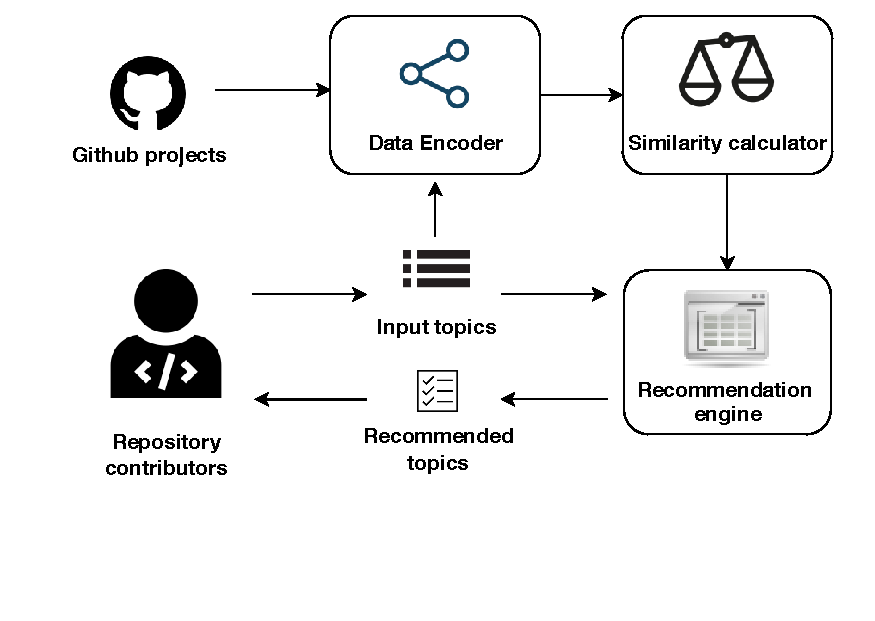
\includegraphics[width=\linewidth]{figs/TopFilter.pdf}
	\caption{Overview of the \TF architecture.}% [??Rename Similarity Computation with Similarity Calculator
	\label{fig:TopFilterArchitecture}
\end{figure}


%This is a preparatory phase for the next steps of the recommendation process. The developer interacts with \TF by sending a request for recommendations that includes the list of topics which she has already included for the repository that she is working on.
%The aforementioned components are singularly described in the next sections. 

In the following subsections, we describe two \TF configurations, namely \TFa and \TFb to recommend relevant topics by incorporating different types of input data. \TFa exploits a collaborative-filtering technique, while \TFb is a combination of both \MNB and \TFa, aiming to improve the prediction performance of the original \MNB approach. % by combining it with \TFa. %\TF can be combined with \MNB to improve. %the collaborative filtering prediction performance.

  %in detail each of the components mentioned above. %In Section~\ref{sec:combined_approach}, 
%Furthermore, based on the proposed architecture, we present an approach to improve \MNB by 

 % shown in Fig. \ref{fig:CrossRecArchitecture} \cite{CROSSREC-DATA}
%\vspace{-.2cm}
%analyzes the input to 
%CrossRec represents the data collected from OSS repositories.
%. The data collected from OSS repositories is converted into a matrix
%A matrix of this type is very sparse since most users give ratings to a small amount of items. 


%\subsection{Recommender}



\subsection{\TFa: Recommending topics using a collaborative-filtering technique} \label{sec:CFRecommendation}

%First \TF represents the relationships among projects\footnote{For the sake of presentation, the terms ``repositories'' and ``projects'' are used interchangeably throughout the paper} and topics retrieved from existing repositories as a graph. %Next, the graph representation are involved to compute similar projects to that under development. Finally, relevant topics are recommended for the input project using a collaborative-filtering technique.

%This section presents the framework to. 

Figure~\ref{fig:TopFilterArchitecture} depicts the architecture conceived to realize the \TF prototype. First, %the \code{Topic Cleaner} component is used to filter out very rare topics according to their frequencies of occurrence over all projects in the initial dataset. Afterwards, 
the \code{Data Encoder} component represents the repositories in the graph format, and then \code{Similarity Calculator} computes similarities among the projects. The \code{Recomme\-ndation Engine} component implements a \emph{collaborative-filtering} technique~\cite{Aggarwal2016,Zhao:2010:UCR:1748610.1749278,NGUYEN2020110460} %,\ it selects top-$k$ similar repository, and performs computation 
to generate a ranked list of \emph{top-N} topics which %.~Finally, a ranked list of topics 
is eventually suggested to the developer. We explain in detail the functionalities of each component as follows.


\subsubsection{Data Encoder} \label{sec:DataEncoder}

%Considering traditional recommender systems for online services, we can identify three main components, namely \emph{users}, \emph{items}, and \emph{ratings} \cite{Sarwar:2001:ICF:371920.372071},\cite{DBLP:conf/rweb/NoiaO15}. 

The mutual relationships among \GH repositories and topics is encoding using a \emph{project-topic matrix}~\cite{Sarwar:2001:ICF:371920.372071}: Each row in represents a project, and each column corresponds to a topic. In this sense, a cell in the matrix is set to 1 if the project in the corresponding row contains the topic in the corresponding column, otherwise the cell is set to 0.

To build the project-topic matrix, raw topics are first pre-process\-ed using various Natural Language Processing (NLP) techniques, such as stemming, lemmatization, and stop words removal. This aims to remove possible syntactical duplicates terms, \eg \textit{document} and \textit{documents}, which are frequent in \GH. Afterwards, the final matrix is constructed by means of the topics obtained through the pre-processing phase. %More specifically, stemming, lemmatization, and stop words are applied on the mined topics.

%the items are represented as columns, and each cell in the matrix corresponds to a rating given by a user for an item \cite{DBLP:conf/rweb/NoiaO15}. Translating this matrix in our domain, users are substitute by projects as well as topics are the possible items to recommend. The resulting \emph{repo-topic ratings matrix} represents possible relationships between these two elements \ie project may include various topics. 

%Pre-processing tasks are performed to transform a metamodel into a feature vector [38], i.e., X = (x1, x2, ..., xL), L is the number of input neurons (see Fig. 2). We illustrate how the Data Extractor 2 works by means of Fig. 4. The Term Extractor E parses terms from the input metamodel. Then, the extracted raw terms are normalized by the NLP Normalizator N that performs the following Natural Language Processing (NLP) steps: (i) stemming (ii) lemmatization, and (iii) stop words removal [23], [55].

%We can denote \emph{project-topic inclusion} relationships as $\ni$. In this matrix, each row represents a project and each column represents a topic. A cell in the matrix is set to $1$ if the topic in the column is included in the project specified by the row, it is set to $0$ otherwise. For the sake of clarity and conformance, we still denote this as a user-item ratings matrix throughout this paper.

For explanatory purposes, we consider a set of four projects $P=\{p_1,p_2,p_3,p_4 \}$ together with a set of topics $L=\{$\emph{t$_1$} = \emph{machine-learning}; \emph{t$_2$} = \emph{javascript}; \emph{t$_3$} = \emph{database}; \emph{t$_4$} = \emph{web}; \emph{t$_5$} = \emph{algorithm}, \emph{t$_6$} = \emph{algorithms}$\}$. Moreover, the \emph{project-topic inclusion} relationships is denoted as $\ni$. By parsing the projects, we discover the following inclusions: $p_1$ $\ni$ $t_1,t_2, t_6$; $p_2 \ni t_1,t_3$; $p_3 \ni t_1 ,t_3, t_4, t_5$; $p_4 \ni t_1,t_2,t_4,t_5$. After the NLP normalization steps, the topics \emph{t$_5$} and \emph{t$_6$} collapse on the same term which is named as \emph{t$_{5}$}. The final project-topic matrix is shown in Table~\ref{tab:repo-topic-matrix}. %is generated to represent inclusions between repositories and topics.

\begin{table}[h!]
	\caption{The \emph{project-topic matrix} of the explanatory example.}
	\begin{tabular}{|p{0.5cm}|p{0.5cm}|p{0.5cm}|p{0.5cm}|p{0.5cm}|p{0.5cm}|p{0.5cm}|} \hline
		& \emph{t$_1$} & \emph{t$_2$} & \emph{t$_3$} & \emph{t$_4$} & \emph{t$_{5}$} \\ \hline
		$p_1$ & 1 & 1 & 0 & 0 & 1 \\ \hline
		$p_2$ & 1 & 0 & 1 & 0 & 0 \\ \hline
		$p_3$ & 1 & 0 & 1 & 1 & 1 \\ \hline
		$p_4$ & 1 & 1 & 0 & 0 & 1 \\ \hline
	\end{tabular}
    \label{tab:repo-topic-matrix}
\end{table}




% Accordingly, the user-item ratings matrix built to model the occurrence of the topic is depicted in Fig.~\ref{fig:UserItemMatrix}.
%====================================================================================================================================
%\footnote{The file \emph{pom.xml} defines all project dependencies with external Maven libraries (\url{https://maven.apache.org/guides/introduction/introduction-to-the-pom.html}) }
%By performing an observation on a data set consisting of more than one thousand GitHub Java projects, we found out that the project-library inclusion matrix is very sparse since most projects contain a limited number of libraries, whereas the total number of libraries included by the projects is pretty large.

%There are two key components: Similarity Computation and Recommendation Engine. The Similarity computation module performs. Based on the list of libraries. Similarity computation is important.
%The former is used to compute similarity between different artifacts, \eg projects, libraries, or even developers. 
%====================================================================================================================================
%is of highly importance. The ability to find most similar projects 
%Similarity computation plays a key role in. Measuring the similarities between developers and software projects is a critical phase for most types of recommender systems \cite{DBLP:conf/rweb/NoiaO15}. Similarities are used as a base by both content-based and collaborative-filtering recommender systems to choose the most suitable and meaningful items for a given item \cite{Schafer:2007:CFR:1768197.1768208}. Failing to compute precise similarities means concurrently adding a decline in the overall performance of these systems. 
%====================================================================================================================================
%Using a recommendation algorithm, CrossRec selects the top most libraries as recommendations. The Recommendation Engine searches for libraries that are included in the similar projects. 
%We also investigate the effect of similarity computation by considering two similarity metrics. 
%Currently, CrossRec supports only GitHub, for future implementation, we expect to include various.
%To incorporate. Based on two premises: Projects use similar libraries to implement similar functionalities. And similar projects use similar set of libraries. To this end, we concentrate on finding a practical solution to represent the relationships between the artifacts, and eventually to compute similarity and cluster OSS projects.
%To compute the similarity between two open software projects. The graph representation allows for different similarity algorithms. In the scope of this paper, we choose the algorithm proposed by \emph{Di Noia et al.} for computing. For future work, other algorithms can also be flexibly included as long as they are suitable for graph.
%: either (i) there are direct links between them; or (ii)
%; or (iii) they are pointed by the same subject with the same property
%For library recommendation, we consider only one property, i.e. \emph{includes} (See Fig. \ref{fig:Graph}). 
%The similarity between $\alpha$ and $\beta$ 
%on a set of properties $P$ is the weighted mean of the values by all properties in $P$ as given below:  
%\begin{equation*}
%VsmSim(\alpha,\beta)=\frac{\sum_{p\in P} \omega_p VsmSim_{p}(\alpha,\beta)}{|P|}
%\end{equation*}
%to compute similarity and finally to provide inputs for a recommender system. 
%====================================================================================================================================
% makes, similarity computation becomes more complicated as many artifacts and several cross relationships prevail.
%As the input for the recommendation process, it is necessary to compute the similarity among software projects. 
%The ability of recommendation is important in the context of mining software repositories. 
%Understanding the similarity between software projects allows for reusing of codes and prototyping, or choosing alternative implementations \cite{10.1109/SANER.2017.7884605}. 
%We see that the ability to measure the similarity between artifacts, \eg projects, code snippets, or even developers, is of highly importance. Meanwhile measuring the similarity between developers and software projects is a critical phase for most types of recommender systems. 
%By considering the analogy of typical applications of RDF graphs and the problem of detecting the similarity of open source projects, in this section we propose. 
%to different open source software projects and 
%an approach that makes use of graphs for representing different kinds of relationships in the OSS ecosystem. 
%One of its applications is to compute similarity computation for supporting recommender systems \cite{DiNoia:2012:LOD:2362499.2362501}.
%With the adoption of the graph representation, it is possible to compute similarity among artifacts exploiting numerous number of graph similarity algorithms. 
%Based on the graph structure, one can exploit nodes, links and the mutual relationships to compute similarity using existing graph similarity algorithms. 
% are incorporated into the similarity calculation
% , given an input project \emph{p}, CrossRec searches for libraries by considering the most similar projects to \emph{p}. 
%====================================================================================================================================
%The rich metadata infrastructure available from the \projectName Knowledge Base is attributed to various artifacts, such as source code, API calls, forum discussions, and bug reports. 
%To this end, we concentrate on finding a practical solution to represent the relationships between the artifacts, and eventually to compute similarity and cluster OSS projects.
%We believe that a homogeneous and formal representation of the intrinsic features of OSS repositories is needed to effectively support project similarity computation.
%In this system, either humans or non-human factors have mutual dependency and implication on the others. 
%A directed graph is defined as a tuple $G=(V,E,R)$, with $V$ being the set of vertices, $E$ being the set of edges and $R$ representing the relationship among the nodes. 
% and Fig. \ref{fig:UserItemMatrix}. 
%sketches the graph representation .  the representation for 
%Specifically, the graph model has been chosen since it allows 
%\todo[size=\tiny, color=green!40]{Nr. 11}
%====================================================================================================================================




\subsubsection{Similarity Calculator} \label{sec:SimilarityCalculator}

%The \code{Recommendation Engine} of \TF works by relying on an analogous user-item ratings matrix. To provide 
%inputs for this module, the first task of \TF is to perform similarity computation on its input data to find the 
%most similar projects to a given project. In this respect, the ability to compute the similarities among projects has 
%an effect on the recommendation outcomes.~Nonetheless, computing similarities among software systems is considered to 
%be a difficult task \cite{McMillan:2012:DSS:2337223.2337267}. In addition, the diversity of artifacts in OSS 
%repositories as well as their cross relationship makes the similarity computation become even more complicated. In OSS 
%repositories, both humans (\ie developers and users) and non-human actors (such as repositories, and libraries) have 
%mutual dependency and implication on the others. The interactions among these components, such as developers commit to 
%or star repositories, or projects include libraries, create a tie between them and should be included in similarity 
%computation.
%
%%Furthermore, the graph structure also facilitates graph kernel methods, which are an effective way to compute similarities \cite{ODMD14a}. 
%%As being inspired by the research from the related Linked Data and Semantic Web field \cite{bizer_linked_2009}, 
%% as done \eg in ~\cite{Nguyen:2015:CRV:2942298.2942305,NDRDSEAA2018}
%% \hl{The representation is inspired by the one presented in}~\cite{NDRDSEAA2018}, however the relationship between projects and libraries is the inverse semantic path, i.e. \texttt{includes} instead of \texttt{isUsedBy}.
%
%
%We assume that a representation model that addresses the semantic 
%relationships among miscellaneous factors in the OSS community is beneficial to 
%project similarity computation. To this end, we consider the community of developers together with 
%OSS projects, topics, and their mutual interactions as an 
%\textit{ecosystem}. We derive a 
%\textit{graph-based} model to represent different kinds of relationships in the OSS ecosystem, and 
%eventually to calculate similarities. In the context of mining OSS repositories, the graph model is a convenient approach since it allows for flexible data integration and numerous computation techniques. 
%By applying this representation, we are able to transform the set of projects and topics shown in Fig.~\ref{fig:UserItemMatrix} into a directed graph as in Fig.~\ref{fig:Graph}.
%%\todo[size=\tiny, color=green!40]{This refers to our SEAA paper} 
%%In Linked Data, an RDF\footnote{RDF 1.1 Concepts and Abstract Syntax: \url{https://www.w3.org/TR/2014/REC-rdf11-concepts-20140225/}} graph is made up of an enormous number of nodes and oriented links with semantic relationships. Thanks to this feature, the similarity of two nodes in a graph can be computed by considering their intrinsic characteristics like neighbour nodes and their mutual interactions \cite{DiNoia:2012:LOD:2362499.2362501,Nguyen:2015:CRV:2942298.2942305}.
%~We adopted our proposed CrossSim approach~\cite{Nguyen:2019:FRS:3339505.3339636},\cite{8498236} to compute the 
%similarities among OSS graph nodes. It relies on techniques successfully 
%exploited by many studies to do the same task 
%\cite{DiNoia:2012:LOD:2362499.2362501},\cite{BRIGUEZ20146467}. Among 
%other relationships, two nodes are deemed to be similar if they point to the same node with the same edge. By looking at the graph in 
%Fig.~\ref{fig:Graph}, we can notice that $p_3$ and $p_4$ are highly 
%similar since they both point to three nodes $topic_{1}, topic_{4}, topic_{5}$.  This 
%reflects what also suggested in a previous work by McMillan \etal 
%\cite{McMillan:2012:DSS:2337223.2337267}, \ie similar projects implement common 
%pieces of functionality by using a shared set of libraries.
%
%
%\begin{figure}[t!]
%	\centering
%	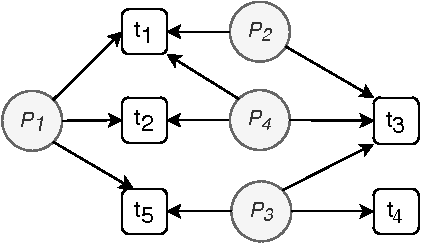
\includegraphics[width=\columnwidth]{figs/Graph.pdf}
%	\caption{Graph representation for projects and libraries.}
%	\label{fig:Graph}
%\end{figure}


%Many recommender systems rely heavily on similarity metrics to suggest suitable and meaningful recommendation for a given  input~\cite{Schafer:2007:CFR:1768197.1768208,Sarwar:2001:ICF:371920.372071,NGUYEN2020110460}. 
%Similarly, 
%The \code{Recommendation Engine} 



%\emph{Similarity Calculator} applies a similarity function on the mentioned project-topic matrix to provide very closest project in a given initial set to the input one. 

%As a result, computing properly this similarity score affects the quality of recommendation outcomes. Nonetheless, computing similarities among topics could be a daunting task. \GH allows any repository owner to add, change, or delete the list of topics that describe his project. This impacts on the stability of the topics, as they can change rapidly over time. In addition, a developer can freely specify the entire set of topics. This makes the similarity computation more complicated, as some topics couldn't have a semantic link with the others. Moreover, we can miss some key relationships depending on the similarity function employed by the calculator. For example, a purely syntactic-based similarity function assign a lower score to the topic pair 3d-graphics even though these two terms are strongly bounded in their meaning.

%a profitable and flexible data representation for enabling numerous computation techniques such as the one defined ~\cite{Nguyen:2019:FRS:3339505.3339636},\cite{8498236} 

This component relies on the information extracted from very similar project to recommend relevant topics to the input repository. We represent a set of projects and their topics in a graph~\cite{Nguyen:2019:FRS:3339505.3339636}, so as to calculate the similarities among the projects.
For instance, Figure~\ref{fig:Graph} depicts the graph-based representation of the project-topic matrix in Table~\ref{tab:repo-topic-matrix} 

Two nodes in a graph are considered to be similar if they share the same neighbors by considering their edges. Such technique has been successfully exploited by many studies to do the same task~\cite{BRIGUEZ20146467} in different domains.

%,\cite{DiNoia:2012:LOD:2362499.2362501}
%By looking at the graph in Fig.~\ref{fig:Graph}, we notice that $p_1$ and $p_2$ share two neighbor nodes, \ie  $topic_{2}$ and $topic_{3}$. %From the graph, we can also learn additional information about the topics themselves. For example, $topic_{3}$ seems a very popular term since is pointed by three different projects. 
%The similarities calculator consider two project nodes $p$ and $q$ as similar in an OSS graph by considering their feature sets. 

Given that $p$ has a set of neighbor nodes ($topic_{1}$, $topic_{2}$,.., $topic_{l}$), the features of $p$ are represented by a vector $\phi=(\phi_{1},\phi_{2},..,\phi_{l})$, with $\phi_{i}$ being the weight of node $topic_{i}$ computed as the \emph{term-frequency inverse document frequency} function as follows: $\phi_{i} = f_{topic_{i}} \times log( \left | P \right | \times a_{topic_{i}}^{-1} )$, where $f_{topic_{i}}$ is the number of occurrence of $topic_{i}$ with respect to $p$, it can be either $0$ and $1$ since there is a maximum of one $topic_{i}$ connected to $p$ by the edge \emph{includes}; $\left | P \right |$ is the total number of considered projects; $a_{topic_{i}}$ is the number of projects connecting to $topic_{i}$ via the edge \emph{includes}.
%\texttt{tf-idf}   of the node 
%\vspace{-.1cm}
%\begin{equation}\label{eqn:TFIDF}
%\phi_{i} = f_{topic_{i}} \times log(\frac{ \left | P \right |}{a_{topic_{i}}})
%\end{equation}
%In the meanwhile, $topic_1$ and $topic_4$ are used only by one project, $p_1$ and $p_3$ respectively. 
%This reflects what also suggested in a previous work by McMillan \etal
%\cite{McMillan:2012:DSS:2337223.2337267}, \ie similar projects implement common
%pieces of functionality by using a shared set of libraries.
\begin{figure}[t!]
\centering
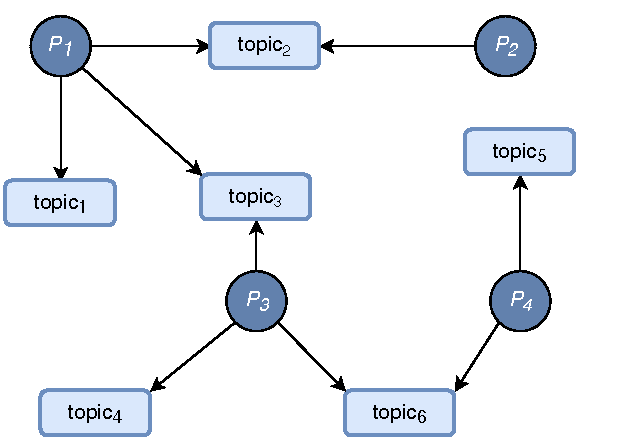
\includegraphics[width=0.8\columnwidth]{figs/graphCFtop.pdf}
\caption{Graph representation for projects and topics.}
\label{fig:Graph}
\end{figure}
%\noindent
%According to Eq.~\ref{eqn:TFIDF}, node $topic_{1}$ in Fig.~\ref{fig:Graph} has a low weight compared to that of other nodes since it is pointed by all four project nodes. In practice, this is comprehensible since \emph{junit:junit} is a very popular dependency and thus it should have a less important role in characterizing a project.
Intuitively, the similarity between two projects $p$ and $q$ with their corresponding feature vectors $\phi=\{\phi_{i}\}_{i=1,..,l}$ and $\omega=\{\omega_{j}\}_{j=1,..,m}$ is computed as the cosine of the angle between the two vectors as given below. %Eventually, the similarity between $p$ and $q$ with their corresponding feature vectors $\phi=\{\phi_{i}\}_{i=1,..,l}$ and $\omega=\{\omega_{j}\}_{j=1,..,m}$ is computed using the cosine similarity function:%\todo[size=\tiny, color=green!40]{Nr. 3}
%\vspace{-.2cm}
% $p$ and $q$ are characterized by using vectors in an $n$-dimensional space, and Eq.~\ref{eqn:VsmSim} measures
\begin{equation} \label{eqn:VsmSim}
sim(p,q)=\frac{\sum_{t=1}^{n}\phi_{t}\times \omega_{t}}{\sqrt{\sum_{t=1}^{n}(\phi_{t})^{2} }\times \sqrt{\sum_{t=1}^{n}(\omega_{t})^{2}}} 
\end{equation}

%\noindent
where $n$ is the cardinality of the set of topics that $p$ and $q$ share in common.% \cite{DiNoia:2012:LOD:2362499.2362501}. %and it is computed using the inner product as follows.







%\textbf{??Intuitive description of eq 2 is needed.}
%====================================================================================================================================
%in which $\omega_p$ is the weight for property $p$ and computed using a genetic algorithm. 
%The hypothesis is based on the fact that the projects are aiming at creating common functionalities by using common libraries.
%In \cite{Jeh:2002:SMS:775047.775126}, SimRank has been developed to calculate similarities based on mutual relationships between graph nodes. Considering two nodes, the more similar nodes point to them, the more similar the two nodes are. In this sense, the similarity between two nodes $\alpha,\beta \in V$ is computed by using a fixed-point function. Given $k \geq 0$ we have $R^{(k)}(\alpha,\beta) = 1$ with $\alpha = \beta$ and $R^{(k)}(\alpha,\beta) = 0$ with $k=0$ and $\alpha \neq \beta$, SimRank is computed as follows:
%
%\begin{equation}\label{eqn:SimRank}
%R^{(k+1)}(\alpha,\beta) = 
%\frac{\Delta}{|I(\alpha)|\cdot|I(\beta)|}\sum_{i=1}^{|I(\alpha)|}\sum_{j=1}^{|I(\beta)|}R^{(k)}(I_{i}(\alpha),I_{j}(\beta))
%\end{equation}
%
%where $\Delta$ is a damping factor ($0 \leq \Delta < 1$); $I(\alpha)$ and $I(\beta)$ are the set of incoming neighbors of $\alpha$ and $\beta$, respectively. $|I(\alpha)|\cdot|I(\beta)|$ is the factor used to normalize the sum, thus forcing $R^{(k)}(\alpha,\beta) \in [0,1]$. 
%
%For the first implementation of CrossSim we adopt SimRank as the mechanism for computing similarities among OSS graph nodes. For future work, other similarity algorithms can also be flexibly integrated into CrossSim, as long as they are designed for graph. %as long as. is able to incorporate various similarity algorithms, 
%\begin{figure}[t!]
%	\centering
%	\includegraphics[width=0.3\textwidth]{figs/SimRank.pdf}
%	\caption{SimRank similarity}
%	\label{fig:SimRank}
%\end{figure}
%====================================================================================================================================
%Equation~\ref{eqn:SimRank} implies that the similarity for two nodes is computed by aggregating the similarity of all possible pairs of their neighbors. 
%We are convinced that the utilization of SimRank is convenient and practical also when various relationships are incorporated into the graph. Given the circumstances, the algorithm needs not be changed since it only works on the basis of nodes and edges. In this sense, 
% \emph{CrossSim} is a versatile similarity tool as it can accept various input features regardless of their format. 
%To study the performance of CrossSim we conducted a comprehensive evaluation using a real dataset collected from GitHub. To aim for an unbiased comparison, we opted for existing evaluation methodologies from other studies of the same type \cite{Lo:2012:DSA:2473496.2473616,McMillan:2012:DSS:2337223.2337267,10.1109/SANER.2017.7884605}. Together with other metrics typically used for evaluations, i.e. \textit{Success rate}, \textit{Confidence},  \textit{Number of false positives}, and \textit{Precision}, we decided to use also \textit{Ranking} to measure the sensitivity of the similarity tools to ranking results. The details of our evaluation are given in the next section. In the first place, it is necessary to compute similarities among projects.
%In this case, the ratings provided by similar users to a target user A are used to make recommendations for A. %The predicted ratings of A are computed as the weighted average values of these “peer group” ratings for each item. 
%From: https://www.sciencedaily.com/releases/2017/12/171206122420.htm
%The recommendation systems at websites such as Amazon and Netflix use a technique called "collaborative filtering."
%To compute the missing ratings, generally there are two ways corresponding to the way we exploit the user-item matrix. In this paper, we investigate both types of collaborative-filtering recommender system: user-based and item-based.
%\paragraph{\textbf{User-based collaborative filtering}}
%One of the most promising such technologies is collaborative filtering [19, 27, 14, 16]. 
%works by filtering or evaluating items using the preferences of other users. 
%In this approach personalized recommendations for a target user are generated using opinions of users having similar tastes to those of the target user. The main assumption in this approach is that users with similar preferences in the past will have similar preferences in the future.
% To compute the missing ratings, there are two main ways, which are basically based on the column-wise and row-wise relationships of the user-item ratings matrix. For \emph{user-based collaborative filtering}. Exploit the relationships among users to deduce the missing ratings. 
%The missing ratings for a given user are computed by exploiting the existing ratings from other similar users. Row-wise computation, among the top most similar projects. 
%====================================================================================================================================
%By online systems, collaborative filtering works by searching for similar. by building a database of preferences for items by users. A new user, Neo, is matched against the database to discover neighbors, which are other users who have historically had similar taste to Neo. Items that the neighbors like are then recommended to Neo, as he will probably also like them. Collaborative filtering has been very successful in both research and practice, and in both information filtering applications and E-commerce applications. However, there remain important research questions in overcoming two fundamental challenges for collaborative filtering recommender systems (Item-based Collaborative Filtering Recommendation Algorithms).
%In addition, collaborative-filtering is considered to be better. 
%from these. calculates similarity between users by comparing their ratings on the same item, and it then computes the predicted rating for an item by the active user
%similar to the active user where weights are the similarities of these users with the target item
%(i.e. the user requiring a prediction) 
%====================================================================================================================================

%A collaborative-filtering recommender system suggests products that customers similar to the customer being considered have already purchased. 

\subsubsection{Recommendation Engine}

%In the context of \TF, we exploit the user-based collaborative-filtering technique for implementing the recommendation engine. 

%Consider the mutual relationships between a project and its topics represented in a graph data structure, we exploit the user-based collaborative-filtering technique to implement \TF's recommendation engine. In this context, we adapted the concept of \emph{rating} to describe the appearance of a specific topic in a project and the employed collaborative filtering techniques aim to find additional similar topics. Moreover, we name the project that needs prediction for topic suggestion as \emph{active project}. Figure~\ref{fig:UserBasedCF} depicts an instance of repo-topic rating matrix where the row $p$ is the active project and an asterisk ($*$) represents a known rating (\ie $1$ if the topics is already included, $0$ otherwise), whereas a question mark ($?$) represents an unknown rating and needs to be predicted.


%\begin{figure}[t!]
%\centering
%%	\vspace{-.4cm}	
%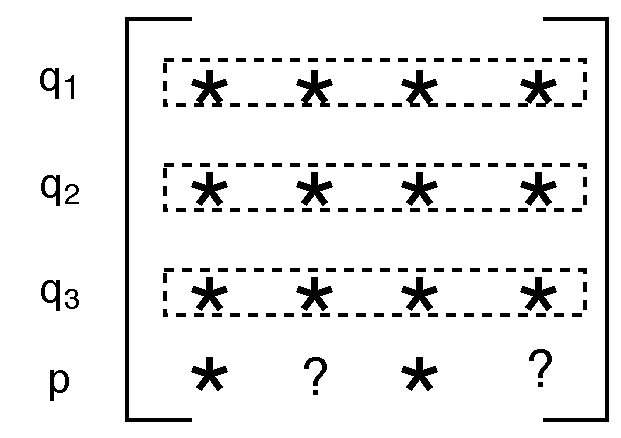
\includegraphics[width=0.55\linewidth]{figs/matrix.pdf}
%\vspace{-.4cm}
%\caption{Deduction of missing ratings~\cite{Zhao:2010:UCR:1748610.1749278}.}% [?? In the previous version there was a rectangle including some of the rows. Isn't?]
%\vspace{-.1cm}
%\label{fig:UserBasedCF}
%\end{figure}

% from the ratings matrix
%using the user-based collaborative-filtering technique



Given an input project $p$, the inclusion of additional topics can be predicted from the projects that are similar to $p$. In other words, \TF predicts topics' presence by means of those collected from the \emph{top-k} similar projects using the following formula~\cite{NGUYEN2020110460}:

%Referring to the example depicted in Figure~\ref{fig:UserBasedCF}, the relationships between the active project $p$ and the similar projects $q_1,q_2,q_3$ are used to compute the missing topic ratings for $p$. 
%The rectangles in Fig. \ref{fig:UserBasedCF} imply that the row-wise relationships between the active project $p$ and the similar projects $q_1,q_2,q_3$ are exploited to compute the missing ratings for $p$.
%The presence of a topic $t$ in project $p$ is deduced by means of the following formula:
%The following formula is used to predict if $p$ should include a topic $t$, \ie~$p \ni t$:%~\cite{DBLP:conf/rweb/NoiaO15}: % the predicted value $r_{p,l}$ is computed
%\vspace{-.2cm}
\begin{equation} \label{eqn:Prediction}
r_{p,t}=\overline{r_{p}}+\frac{\sum_{q \in topsim(p)}(r_{q,t}-\overline{r_{q}})\cdot sim(p,q) }{\sum_{q \in topsim(p)} sim(p,q) } %\left | P \right |
\end{equation}

\noindent
where $\overline{r_{p}}$ and $\overline{r_{q}}$ are the mean of the ratings of $p$ and $q$, respectively; $q$ belongs to the set of \emph{top-k} most similar projects to $p$, denoted as $topsim(p)$; $sim(p,q)$ is the similarity between the active project and a similar project $q$, and it is computed using Equation \ref{eqn:VsmSim}. %For a testing project $p$, $\overline{r_{p}}$ is equal to $1$ since the ratings for all testing libraries are $1$.




%\subsection{Recommendation Engine} \label{sec:RecommendationEngine}
%\PN{Please reprhare this section}
%The representation using a user-item ratings matrix allows for the computation of missing ratings \cite{Aggarwal2016},\cite{DBLP:conf/rweb/NoiaO15}. Depending on the availability of data, there are two main ways to compute the unknown ratings, namely \emph{content-based} \cite{Pazzani2007} and \emph{collaborative-filtering} \cite{Miranda:2008:ICF:1486927.1487083} recommendation techniques. The former exploits the relationships among items to predict the most similar items. The latter computes the ratings by taking into account the set of items rated by similar customers. There are two main types of collaborative-filtering recommendation: \emph{user-based} \cite{Zhao:2010:UCR:1748610.1749278} and \emph{item-based} \cite{Sarwar:2001:ICF:371920.372071} techniques. As their names suggest, the user-based technique computes missing ratings by considering the ratings collected from similar users. Instead, the item-based technique performs the same task by using the similarities among items \cite{Cremonesi:2008:EMC:1468165.1468327}.
%
%In the context of \CR, the term \emph{rating} is understood as the occurrence of a library in a project and computing missing ratings means to predict the inclusion of additional libraries. The project that needs prediction for library inclusion is called the \emph{active project}. By the matrix in Fig. \ref{fig:UserBasedCF}, $p$ is the active project and an asterisk ($*$) represents a known rating, either $0$ or $1$, whereas a question mark ($?$) represents an unknown rating and needs to be predicted.
%
%%Because of the above assumptions, the collaborative filtering algorithm is based on the comparison of one user’s behavior with other user’s behavior, to find his nearest neighbors, and according to his neighbor’s interests or preferences to predict his interests or preferences.
%
%\begin{figure}[t!]
%	\centering
%	%	\vspace{-.4cm}
%	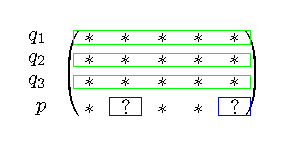
\includegraphics[width=0.7\linewidth]{figs/UserBasedCF.pdf}
%	\vspace{-.4cm}
%	\caption{Computation of missing ratings using the user-based collaborative-filtering technique~\cite{Zhao:2010:UCR:1748610.1749278}.}% [?? In the previous version there was a rectangle including some of the rows. Isn't?]
%	\vspace{-.1cm}
%	\label{fig:UserBasedCF}
%\end{figure}
%
%%\CR employs a collaborative-filtering technique   based on the similar model applied in e-commerce systems
%
%Given the availability of the cross-relationships as well as the possibility to compute similarities among projects using the graph representation, we exploit the user-based collaborative-filtering technique as the engine for recommendation \cite{Linden:2003:ARI:642462.642471,Zhao:2010:UCR:1748610.1749278}. Given an active project $p$, the inclusion of libraries in $p$ can be deduced from projects that are similar to $p$. The process is summarized as follows: % \cite{Cacheda:2011:CCF:1921591.1921593}:
%%In particular, the user-based collaborative-filtering technique predicts a missing rating by considering the most similar projects to $p$. 
%
%%%The engine first searches for similar projects and then computes missing ratings as a weighted average of the ratings of the items by projects .
%%According to [16, 15], item-based CF algorithms provide better performance and quality than user-based ones. Afterwards the unknown ratings are computed by considering the libraries included in these projects. In this paper, the user-based technique is utilized. 
%
%\begin{itemize} 	
%	\item Compute the similarities between the active project and all projects in the collection;
%	\item Select \emph{top-k} most similar projects; and %a subset of the users (neighborhood) according to their similarity with the active user;
%	\item Predict ratings by means of those collected from the most similar projects.
%\end{itemize} 
%
%The rectangles in Fig. \ref{fig:UserBasedCF} imply that the row-wise relationships between the active project $p$ and the similar projects $q_1,q_2,q_3$ are exploited to compute the missing ratings for $p$. The following formula is used to predict if $p$ should include $l$, \ie~$p \ni l$~\cite{DBLP:conf/rweb/NoiaO15}: % the predicted value $r_{p,l}$ is computed
%%\vspace{-.2cm}
%\begin{equation} \label{eqn:Prediction}
%r_{p,l}=\overline{r_{p}}+\frac{\sum_{q \in topsim(p)}(r_{q,l}-\overline{r_{q}})\cdot sim(p,q) }{\sum_{q \in topsim(p)} sim(p,q) }  %\left |  P \right |  
%\end{equation}
%
%\noindent
%where $\overline{r_{p}}$ and $\overline{r_{q}}$ are the mean of the ratings of $p$ and $q$, respectively; $q$ belongs to the set of \emph{top-k} most similar projects to $p$, denoted as $topsim(p)$; $sim(p,q)$ is the similarity between the active project and a similar project $q$, and it is computed using Equation \ref{eqn:VsmSim}. %For a testing project $p$, $\overline{r_{p}}$ is equal to $1$ since the ratings for all testing libraries are $1$. 


%\subsection{CrossRec in Action}
%\label{sec:inaction}
%In the context of the EU H2020 CROSSMINER project\footnote{\url{https://www.crossminer.org}}, we integrated \CR 
%into Eclipse as shown in Fig.~\ref{fig:IDE}. 
%The figure describes a development of an explanatory scenario where a 
%	developer is improving a software project, named \textit{aethereal} hereafter, 
%	by replacing some existing source code with features provided by third-party 
%	libraries. The goal of such changes is to make the code easier to be understood 
%	and evolved. The project is a command line tool written in Java that aims at 
%	supporting the automatic generation of cross-projects migration dependencies 
%	graph. To this aim \textit{aethereal} distinguishes between clients and 
%	libraries: both clients and libraries are Maven artifacts, and clients are 
%	defined as artifacts that use a specific  library available on the Maven 
%	repository.
%
%We explain how \CR helps the developer evolve the  \code{build} method of the class \code{MavenDataset} as follows.
%	Such a  method computes a dependency matrix between client versions and libraries. The initial implementation of the \code{build} method prints the logging information to the console by using Java I/O facilities (\ie~\code{System.out.println} and \code{System.err.println}) \circled{1}.
%	The \CR tool displays the list of third-party libraries currently being included \circled{2}, and prompts a list of recommended libraries \circled{3}. The list of recommended libraries highlights the suggestion for using a logging library, \ie~\code{slf4j}\footnote{\url{https://www.slf4j.org/}} or \code{{commons-logging}\footnote{\url{https://commons.apache.org/proper/commons-logging/}}}. Then, a possible m igration to \code{slf4j} is shown \circled{4}, where the \code{System.out.println} and \code{System.err.println} invocations are replaced by \code{slf4j} \code{logger.info} and \code{logger.debug} calls, respectively.
%
%\begin{figure}[t!]
%	\centering
%	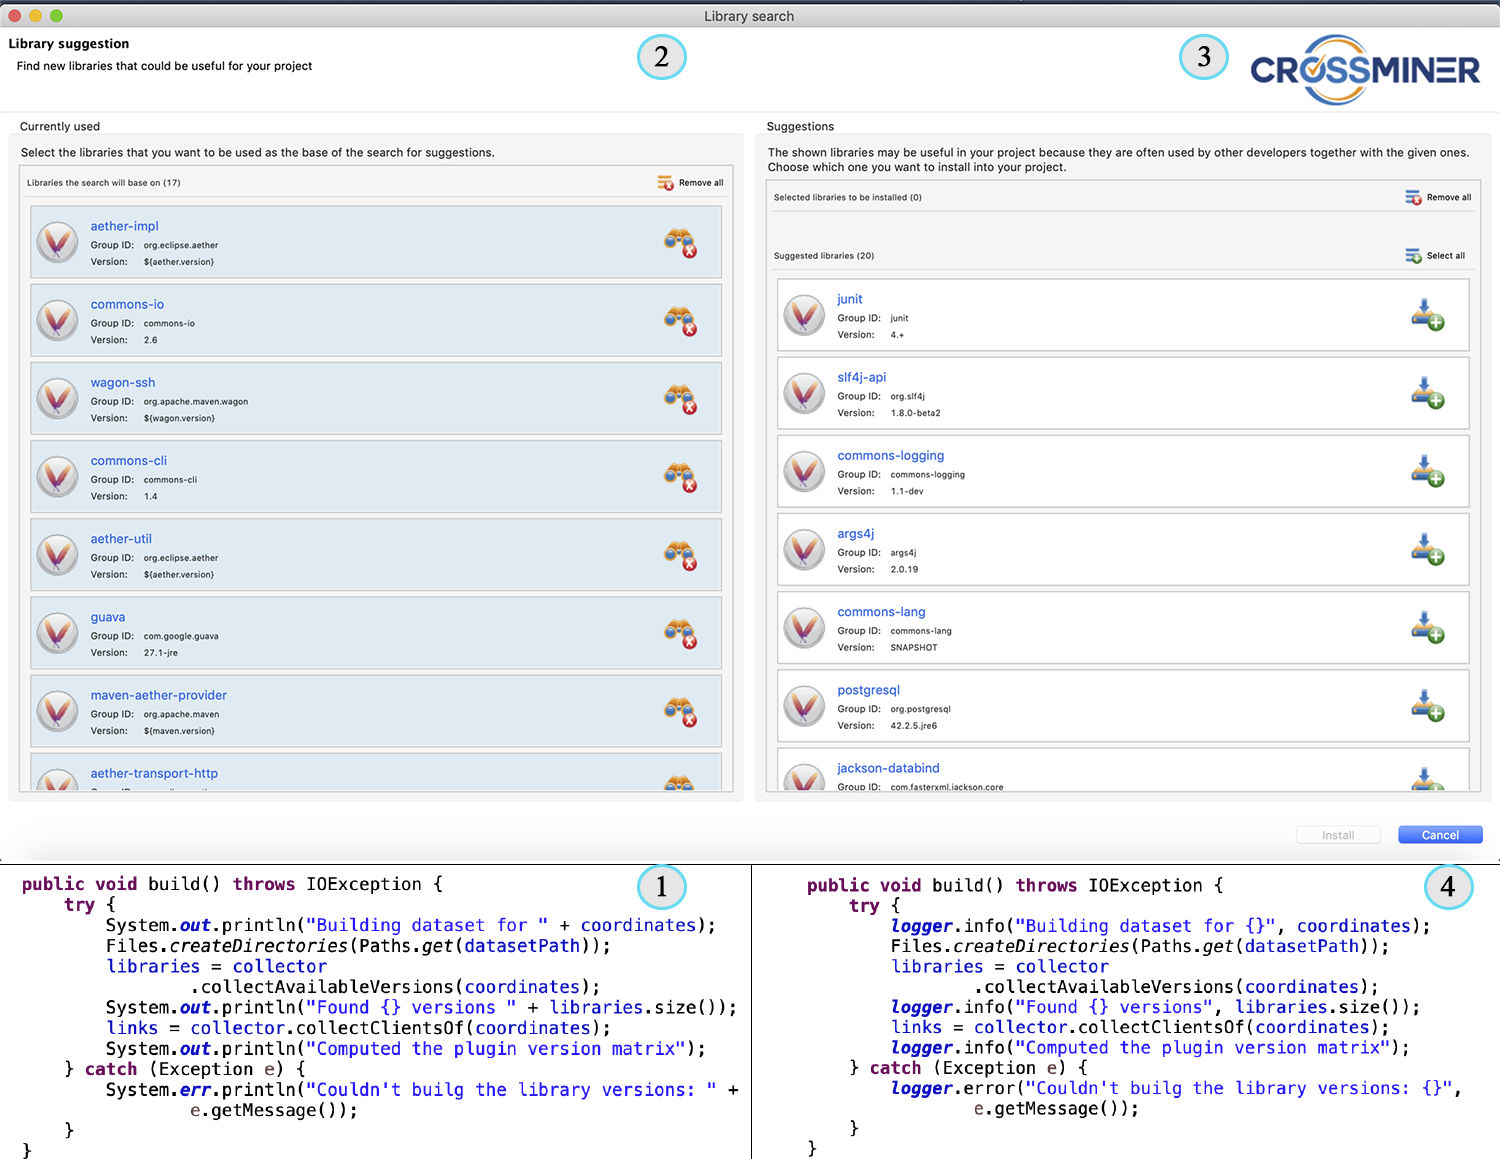
\includegraphics[wid\\th=\textwidth]{figs/CrossRecIDE.png}
%	%\vspace{-.3cm}
%	\caption{\CR IDE.}
%	\label{fig:IDE}
%	\vspace{-.3cm}
%\end{figure}
%
%
%
%In its current version, \CR recommends a set of libraries to developers, however it is likely that only some of the suggestions will result as useful for them. While the current version of \CR is unable to capture developers' feedback, it is possible to re-train again and obtain new recommendations based on the up-to-date code base.



\subsection{\TFb: Improvement of \MNB} \label{sec:combined_approach}

%So far, we have described \TF as a stand-alone recommender system by describing its constituent components. To highlight its flexibility in a different context, we propose an approach to improve \MNB. 

As already mentioned in Section~\ref{sec:Background}, though \MNB works in practice, it has its own limitations. First, it can recommend only featured topics which account for a small fraction of all possible terms. %, which in turn can be restricted because of antonymous terms, \eg programming languages. 
Second, given that a repository already includes all suggested topics, \MNB is not able to recommend new ones. %The second major limitation is the underlying structure needed for the training phase. 
Moreover, the tool requires a \emph{balanced} dataset, \ie each topic must have a similar number of \RM files, and this is hard to come by in practice as topics are generally heterogeneous. With \TFb, we attempt to improve \MNB by combining it with the collabora\-tive-filtering technique presented in the previous subsection. The set of featured topics predicted by the MNB model is used as input to feed \TF which then runs the filtering process to deduce the inclusion of new topics.

Figure~\ref{fig:entangled} depicts an overview of the \TFb configuration: a list of featured topics computed by \MNB using README files is fed as input for \TFb, which computes a list or ranked topics, including also non-featured ones. Finally, a list is generated by combining the topics computed by \TFb with the top-N featured ones computed by \MNB, and recommended to developers.


\begin{figure}
	\centering
	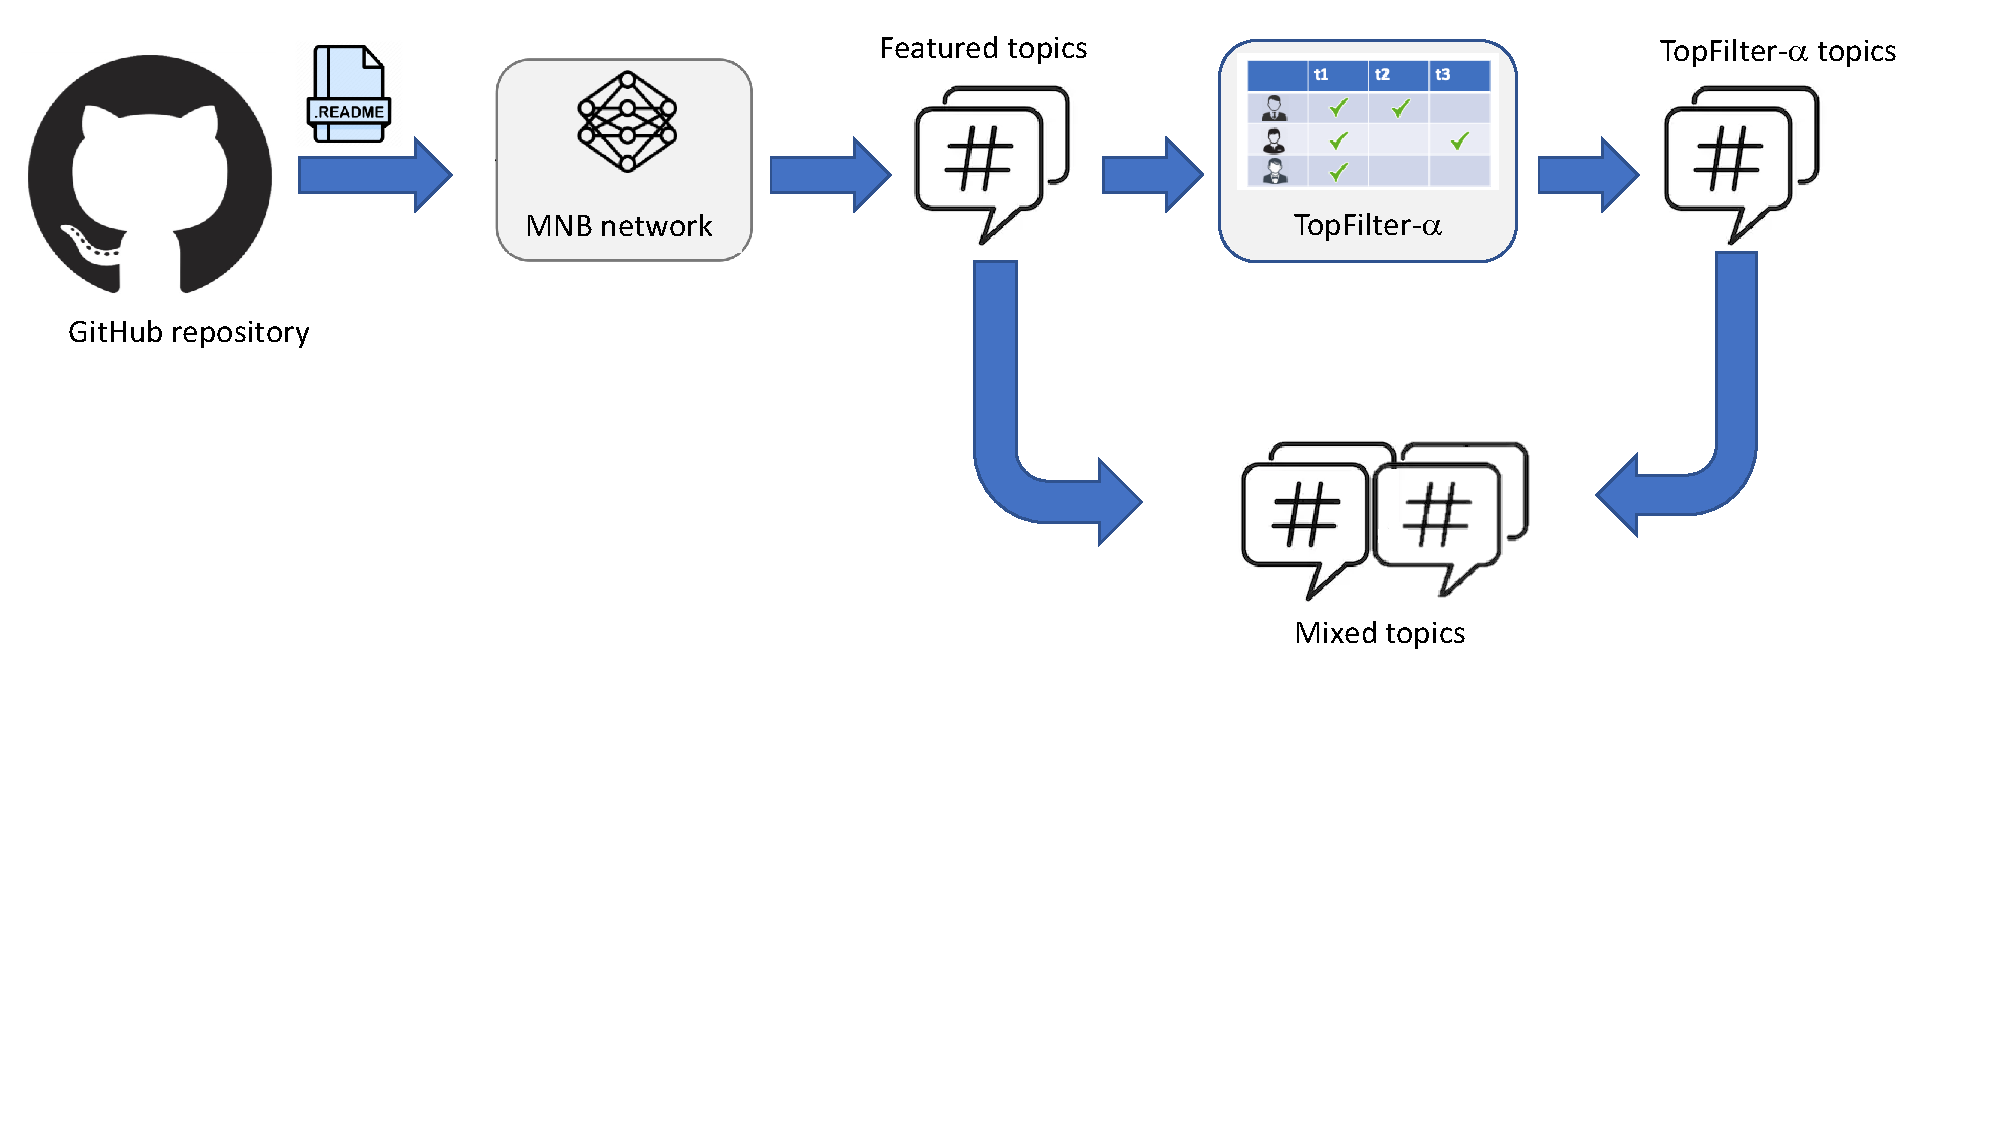
\includegraphics[width=\linewidth]{figs/entangled.pdf}
	\caption{Overview of the combined approach.}
	\label{fig:entangled}
\end{figure}

%as follows. %\emph{entangle} our tool with the MNB network using it as a black box. 
%In particular, we show how \TF can be combined with other recommender systems that use a different mining strategy.

%As mentioned before, this recent work using the \RM file of a repository to predict featured topics. It involves all the standard techniques employed in the ML domain \ie textual engineering, feature extraction, and training phase. Given a \RM file, the approach computes vectors using the TF-IDF weighting scheme to extract features. Then, the model is trained to retrieve the most probable featured topics according to the multinomial distribution with the Naive Bayesian assumption. The outcomes are evaluated using the ten folder validation process.
%, resulting in \TFb

%The aim of this kind of analysis is to evaluate \TF capability using a well-founded technique in the literature.  can help improve \MNB 
We assume that \TFb is beneficial in the following aspects:
\begin{itemize}
	\item It is able to recommend non-featured topics, which are selected from similar repositories, independently from their nature;
	\item \TFb recommends topics by iterating over refining steps: once we select some topics from the recommended ones, \TFb can discover new topics using the selected ones as new input;
	\item \MNB does not provide additional recommendations given that the suggested topics are already included. As we will see in Section~\ref{sec:EXP1}, \TFb considerably improves the performance when more topics are incorporated as input.
\end{itemize}

%The experiments conducted 
In the following sections, we introduce the experiments conducted to evaluate the performance of \TF, \MNB, and the combined approach by comparing the accuracy and coverage metrics.

